
% Master LaTex file for gyarb

% Shortcuts
% C-c C-c compile
% Compile
% 1: pdflatex garb_bokma.tex, 2: biber garb_bokma, 3: pdflatex garb_bokma.tex


\documentclass[11pt]{article}

% packages
\usepackage[margin=1in]{geometry}
\usepackage[backend=biber]{biblatex}
\usepackage{graphicx}
\usepackage{wrapfig}
\usepackage{csvsimple}

% settings
\addbibresource{garb_bibl/garb_bibl.bib}

% title
\title{Gymnasiearbete {\LaTeX} dokument}
\author{Otte Bokma}

% document
\begin{document}

\begin{titlepage}

  \begin{center}
    \huge{Predicting long term effects of TBI using machine learning}
    \\[1cm]
    \large{Using agglomerative clustering as a machine learning method to try to classify long term effects of traumatic brain injury}
  \end{center}
\end{titlepage}

\section*{Sammanfattning}

\subsection*{Bakgrund}

Hjärnskakningar är skador som är mer eller mindre vanliga beroende på en persons dagliga aktiviteter. De framkommer framför allt bland idrottare inom vissa sporter, emepelvis boxning, amerikansk fotboll och ishockey. Hjänskakningar är även en relativt vanlig skada vid trafikolyckor (whiplash). Det finns dock väldigt många olika former av hjänskakningar och symptomen varierar på både lång och kort sikt väldigt mycket mellan fallen. Att förutsäga de långvariga symptomen kan vara väldigt svårt. En del personer påverkas nästan inte medan andra kan få problem som varar i många år.\\
\\
Artificiell intelligens är något som används väldigt mycket i nuläget för en mängd olika saker. Artificiell intelligens har visat sig kunna användas väldigt effektivt för bland annat denna typ av uppgift, att identifiera eller förutsäga något utifrån olika variabler. Det skulle alltså vara tänkbart att artificiell intelligens till viss mån skulle kunna identifiera möjliga långvariga symptom av en hjärnskakning utifrån de kortvariga symptomen.

\subsection*{Metod och Resultat}

\subsection*{Slutsats}

\section*{Abstract}

\subsection*{Background}

Traumatic Brain injury (TBI) is a condition with varying presence depending on a persons daily activities. Above all TBI shows among athletes of some sports, such as boxing, american football and icehockey. TBI is also a relatively common injury in traffic accidents(, often in connection with a whiplash type injury). There are many different types of TBI and the sypmtoms can vary widely in both long term and short term. To predict the long term effects of TBI can therefore be very hard. Som people have almost no long term symptoms whilst others may have sypmtoms years after the accident occured.\\
\\
Nowadays machine learning is used widely and has many different kinds of application. Machine learning has been shown to be very suitable for this type of application in a lot of instances, to identify or pedict something based on a set of variables. Thus it could be conceivable that one could to at least some extent identify possible long term effects based on the short term symptoms of a TBI patient using machine learning.\\
\\
*
Traumatic brain injury (TBI) is a condition that can be quite hard to diagnose and even if it is diagnosed the long term effects and symptoms can be hard to identify. Machine learning and artificial intelligence has in recent times gained popularity as is gives a way of identifying and predicting things that humans can not always do. As for TBI there is a lot of data to be collected about a patients health status at the time of being examined. This data is unfortunately quite hard for humans to interpret. Using machine learning to interpret this data is a great opportunity to harness the power of data classification that is machine learning.
*

\subsection*{Method and Findings}
The type of machine learning algorith used is a support vector machine (SVM), a type of approach developed in the 1990s. SVMs are shown to perform well in many different settings and are considered to be one of the best classifiers to use without doing considerable optimization for a specific classification problem.\\
\\
The classification was conducted by separating data values into features (used for predicting the label) and labels (predicted using features). The features and labels are then divided into training data and test data. In this case the training data consists of 80\% of all data and the test data consists of 20\%. The training data is what the algorithm uses to make a model of a function by which is considers the data to be separable, then this model is tested on the test data and scored by the precentile of correct  classifications.\\
\\
The separation of data into training and test data is done for each iteration of running the algorithm and each time the datapoints are separated the datapoints are used for each group are randomize. Thus the data used for training and prediction is not the same every time which means that also the results vary for each iteration of running the algorithm. To make the results more reliable the program runs 3000 iterations for the division of the data, and the algorithm. The score for each iteration is calculated and added to a variable, after which the total sum is divided by the number of iterations to get the average score.\\
\\
Results from a few of the iterations are also analyzed manually to see what kind of predictions the algorithm makes. A great part of the label classes are concentrated to just one or two of the classes, meaning that the algorithm can get a score that is quite high by just classifying all labels into one or two classes.

\subsection*{Conclusion}

\newpage
\tableofcontents
\newpage
\section{Introduction}

\subsection{Purpose}

\subsection{``Frågeställning''}

\begin{enumerate}
  \item{How accurately can the Marshall and Rotterdam classifications be predicted with data of the injuries a patient has sufferd.}
  \item{Can a correlation between genetic factors and patient outcome be found using machine learning(GOSE, PTSD)}
  \item{How well do the Marshall and Rotterdam classifications predict the score of the Extended Glasgow Outcome Scale (GOSE)}
\end{enumerate}

\section{Method}
\subsection{Support Vector Machines}
The support vector machine, or SVM, is a generalization of a classifier called the \textit{maximal margin classifier}. This classifier however, can not be applied to most datasets as it requires classes to be separable by a linear boundary. With the use of the \textit{support vector classifier}, which is an extension of the of the maximalmargin classifier, SVMs become applicable to more datasets. The \textit{support vector machine} is a further extension of the \textit{support vector classifier} that accomomodates for class boundaries that are non-linear. Even further extensions can be made to the \textit{support vector machine} to make it applicable to more than two classes.\cite{jamesSupportVectorMachines}

It is important to distinguish between the \textit{maximal margin classifier}, \textit{support vector classifier} and \textit{support vector machine}, as not to confuse them with eachother.\cite{jamesSupportVectorMachines}\\
\\
\subsubsection{Maximal Margin Classifier}
A classifier that divides data into two classes with a linear line: The the maximum margin.

\subsubsection{Support Vector Classifiers}

\subsubsection{Support Vector Machines}

\subsubsection{SVMs with More than two Classes}

\subsubsection{Kernels}
Kernels are similarity functions. A similarity functions objective is to calculate the similarity between objects. Using a kernel means that we can add dimensions so that the data gets separable into classes. The use of a kernel implies the use of a kernel function, that enables the use of high-dimensional space without needing to compute the coordinates of the thata in that space. Instead it calculates the inner (dot) product for all pairs of images of data.\\
\\
The type of kernel used defines what kind of function is used to make the model for separating the data into different classes.\\
\\
Image\\
\\
\large{Linear kernel}\\
A linear kernel

\large{Radial basis function kernel}\\

\large{Polynomial kernels}

\section{Score}

\subsection{Marshall CT Score}
The Marshall classification of traumatic brain injury, or Marshall CT score, is a metric used for classification of traumatic brain injury. The classification system is a CT scan derived metric that has shown to predict patient outcome in cases og traumatic brain injury.\cite{gaillardMarshallClassificationTraumatic}\\
\\
The Marshall system divides patients into six categories.
Patients are divided into six categories (I to VI) by the Marhall system. Categorization is done on the basis of a non-contrast CT scan of the brain. The severity increases with the numbers, VI being the most severe, and thus the higher numbers have worse prognosis and survival. The system focuses mostly on two features: Degree of swelling, which is determined by midline shift and/or compression of basal cisterns, and the presence and size of contusions/haemmorages that are referred to as ``high or mixed density lesions'' in the classification.\cite{gaillardMarshallClassificationTraumatic}\\
\\
The scored elements in the Marshall classification are:

\begin{itemize}
\item{degree of basal cistern compression}
\item{degree of midline shift}
\item{presence and size of contusions/heaemorraghes}
\end{itemize}

The classifications of the Marshall CT score are the following:

\begin{enumerate}
\item{Diffuse Injury I}
  \begin{itemize}
    \item{no visible intracranial pathology}
  \end{itemize}
\item{Diffuse Injury II}
  \begin{itemize}
   \item{midline shift 0 to 5mm}
    \item{basal cisterns reamin visible}
    \item{no high  or mixed density lesions $>25 cm^3$}
  \end{itemize}
\item{Diffuse Injury III}
  \begin{itemize}
    \item{midline shift 0 to 5mm}
    \item{basal cisterns compressed or completely effaced}
    \item{no high or mixed density lesions $>25cm^3$}
  \end{itemize}
\item{Diffuse Injury IV}
  \begin{itemize}
    \item{midline shift >5 mm}
    \item{no high or mixed density lesions $>25cm^3$}
  \end{itemize}
\item{Diffuse Injury V}
  \begin{itemize}
    \item{any lesion evacuated surgically}
  \end{itemize}
\item{Diffuse Injury VI}
  \begin{itemize}
    \item{high or mixed density lesions $>25cm^3$}
    \item{not surgically evacuated}
  \end{itemize}
\end{enumerate}

\subsection{Rotterdam CT Score}
The Rotterdam CT score of traumatic brain injury is a classification purposed for improving prognostic evalutaion for patients admitted with acute trumatic brain injuries. The Rotterdam system is more recent than the Marshall classification of traumatic brain injury which tries to address some of the limitations that the older Marshall system has. Instead of having three independently scored elements the Rotterdam system has four, and one of the elements is slightly different from the Marshall system.\\
\\
The scored elements in the Rotterdam classification are:

\begin{itemize}
\item{degree of basal cistern compression}
\item{degree of midline shift}
\item{epidural haematomas}
\item{intraventricular and/or subarachnoid blood}
\end{itemize}

The classification of the Rotterdam CT score is scored by the following system:

\begin{itemize}
\item{basal cisterns}
  \begin{itemize}
    \item{0: normal}
    \item{1: compressed}
    \item{2: absent}
  \end{itemize}
\item{midline shift}
  \begin{itemize}
    \item{0: no shift or $\geq$ 5mm}
    \item{1: shift $>$ 5mm}
  \end{itemize}
\item{epidural mass lesion}
  \begin{itemize}
    \item{0: present}
    \item{1: absent}
  \end{itemize}
\item{intraventricular blood or traumatic SAH}
  \begin{itemize}
    \item{0: absent}
    \item{1: present}
  \end{itemize}
\end{itemize}
The final score is the sum of the scores for each individually assessed element + 1.\\
\\
The Rotterdam CT score has probablility of mortality at six months post-injury for each score.\\
\begin{enumerate}
  \item{0\%}
  \item{7\%}
  \item{16\%}
  \item{26\%}
  \item{53\%}
  \item{61\%}
\end{enumerate}

\subsection{Extended Glasgow Outcome Scale}
The GOS-E, or GOSE, is an extension developed to the original Glasgow outcome scale (GOS) in 1981 to address some of its limitations. The original GOS has five categories, these are extended to eight in the GOS-E. In 1998 a questionnare with guidelines was provided to improve the reliability of the GOS ans GOS-E ratings\cite{GOSEExtendedGlasgow}.\cite{ExtendedGlasgowOutcome}\\
\\
The categories of the GOS-E are:
\begin{itemize}
  \item{Dead}
  \item{Vegetative State}
  \item{Lower Severe Disability}
  \item{Upper Severe Disability}
  \item{Lower Moderate Disability}
  \item{Upper Moderate Disability}
  \item{Lower Good Recovery}
  \item{Upper Good Recovery}
\end{itemize}



\section{Factors}

\subsection{Injuries}

\subsubsection{CT Brain Pathology}
Brain pathology is disease in the brain, CT brain pathology is the study of brain diseases which can be found by compudet tomography (CT).
The data indicates whether any brain pathology could be indicated via a CT scan.

\subsubsection{CT Skull Fracture}
The cranial portion of the skulle consists of eight bones. A skull fracture is a fracture or break in any one of these bones. A skull fracture may cause underlying structures such as membranes, blood vessels and brain to be damaged.\cite{SkullFracture2020}\\
\\
If no part of skull bone causes damage to tissue around it a skull fracture in itself is not that significant. Skull fractures can occur without there being any other physical or neurological damage. It is however very indicative of a significant amount of force applied to the head if there is a skull fracture in healthy bone. When a skull fracture is caused to healthy bone it isvery likely that this person has suffered a concussion, wether with or without loss of conciousness.\cite{SkullFracture2020}\\
\\
Compound fractures
(major) Types of skull fractures:

\subsubsection{CT Skull Base Fracture}
Skull base fractures, often referred to as balas or basilar skull fractures, is the break of a bone in the base of the skull. The bones the break can occur in are the temporal bone, occipital bone, sphenoid bone, frontal bone, or ethmoid bone. Depending on where the fracture has occured thefractures are divided into anterior, central or posterior fractures. For a skull base fracture to occur it generally requires a significant amount of trauma. The diagnosis of basal skull fractures is mostly done by a CT scan.\cite{BasilarSkullFracture2021}\\
\\
Symptoms that can be caused by basal skull fractures include bruising behind the ears, bruising around the eyes, blood behind the ear drum, and cerebrospinal fluid (CSF) leak, which occurs in about 20\% of cases, that may cause fluid to leak from nose or ears. Other possible effects are cranial nerve or blood vessel injury and about 14\% of cases cause in meningitis, which is the inflammation of the protective membranes that cover the brain and spial chord.\cite{BasilarSkullFracture2021} *WRITE ABOUT MENINGITIS SYMPTOMS*\\
\\
\begin{figure}[ht]
  \centering
  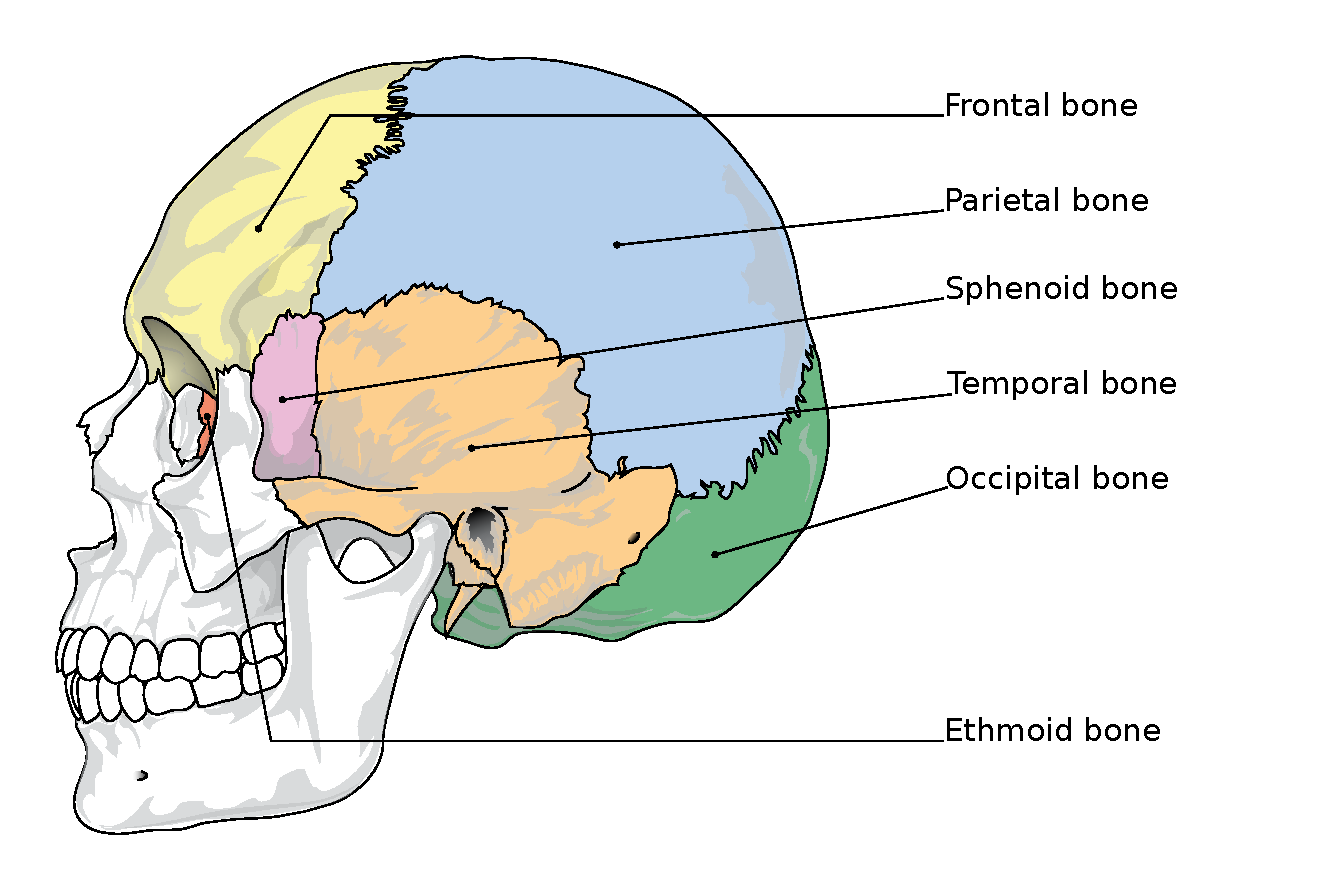
\includegraphics[width=12cm]{graphics/cranial_bones.pdf}
  \caption{Figure showing what bones may be involved in a basal skull fracture}
\end{figure}

\subsubsection{CT Facial Fracture}
\subsubsection{CT Epidural Hematoma}
\subsubsection{CT Subdural Hematoma}
\subsubsection{CT Subarachnoid Hemorrhage}
\subsubsection{CT Contusion}
\subsubsection{CT Midline Shift}
\subsubsection{CT Cisternal Compression}

\subsection{Genetic}

\subsubsection{catechol-O-methyltransferase gene}
The catechol-O-methyltransferase (COMT) gene is a gene which variations affect dopamine levels in the prefrontal cortex\cite{COMTSNPedia}. The gene codes for catechol-O-Methyltransferase, an enzyme that breaks down dopamine in the prefrontal cortex\cite{Rs4680SNPedia}.
\subsubsection{rs4680}
rs4680, also sometimesreferred to as Val158Met, Val108/158Met or G1947A, is a single-nucleotide polymorphism (SNP) in the COMT gene. The nucleotide substitution between A and G results in changing the amino acid at codon 158 from valine, for genotype G;G, to methionine, for genotype A;A. The A/Met allele makes a change in the enzyme which has been shown to have lower enzymatic activity (because of thermoinstability).\cite{Rs46802020}\\
\\
The activity is supposedly only 25\% of the enzyme coded for in the case of the G/Val allele. The difference in levels of dopamine in the frontal cortex caused by the SNP is in some cases named the warrior/worrier hypothesis. People with the Met allele are described as ``worriers'' and considered to be more ``exploratory'', a description that is not defined in any exact way\cite{ExploratoryBehaviorOverview}, than people with the Val allele. The Val allele carriers are described as ``warriors'' and considered less ``exploratory''. Some more tangible differences that have been observed and are thought to be caused by the difference in dopamine levels are lower pain threshold, enhanced vulnerability to stress, and higher efficiency for processing information under most conditions for the Met allele, carriers having higher dopamine levels, and higher pain threshold, better stress resiliency, and a modest reduction in executive cognition performance under most conditions for the Val allele, carriers having lower dopamine levels.\cite{Rs4680SNPedia}
\cite{Rs4680SNPedia}

\subsubsection{rs6277}
\subsubsection{rs3219119}
\subsubsection{rs11604671}
\subsubsection{rs4938016}
\subsubsection{rs1800497}

\section{Results}
The support vector machine is a supervised learning method which means the data has to be split up into training and testing data. This split affects the results when the classification is socored. Using different training data means the classes will be different and thus it will classify the data differently depending on the training data. For this reason the accuracy of the function varies so 3000 iterations have been run for all the results, except where the number of iterations is stated.
\subsection{Injury Factors}
*Run results for SVM on 3 kernels, balanced \& unbalanced, predicting Marshall and Rotterdam CT scores. Run 3000/5000 iterations each time.*
Initial result: Quite good, about 89\% right for Marhsall and about 70\% for Rotterdam, also many of those not being 1/2 => GOOD

\subsection{Genetic Factors}
*Run results for SVM on 3 kernels, balanced \& unbalanced, predicting GOSE and PTSD scores. Run 3000/5000 iterations each time.*
Initial result:

\subsection{Combined Factors}
*Run results for SVM on 3 kernels, balanced \& unbalanced, predicting Marshall and Rotterdam CT scores. Run 3000/5000 iterations each time.*
Initial result: Running with both injuries and genetics as factors for the Rotterdam score the precentage actually increases a little, not much but it does seem to improve even though the number of observations decreases. For the Marshall score it does not seem to make any difference.

\section{Discussion}
The classification choice problem:\\
For classification of TBI it is intended to get a prediction of what class an injury is and how it affects the person in question. This leads to a problem that is: What are the classes? The purpose of this kind of algorithm would be to classify the patients into groups but the problem is defining a group.\\
\\
The dataset that is used has a quite limited sample size. The number of samples being so low means that there is a low chance of there being great consistency to be found in the data. What also affects the results is an inherent flaw in the way the research has been conducted. As the intention of a program like this is to find patterns where we humans cannot find them it is important that the program get raw data about something. In this case the data has already been processed and interpreted by humans which means that the program only has access to data that is already processed by humans. If humans cannot, using their observations, with certainty say what has been damaged in the brain and what this will lead to the data that the humans collect will be flawed in this same way.\\
\\
To increase chances of success in a project like this it would be advised to use data that has in no way been interpreted by humans. Imaging of the brain is what would be most easily accessible and also seems to be the most relevant for this purpose. Then letting an artificial intelligence algorithm try to classify them into subgroups. Although even this method suffers from the classification choice problem.\\
\\

\section{Bibliography}

\printbibliography

\end{document}